%%%%%%%%%%%%%%%%%%%%%%%%%%%%%%%%%%%%%%%%%
% FRI Data Science_report LaTeX Template
% Version 1.0 (28/1/2020)
% 
% Jure Demšar (jure.demsar@fri.uni-lj.si)
%
% Based on MicromouseSymp article template by:
% Mathias Legrand (legrand.mathias@gmail.com) 
% With extensive modifications by:
% Antonio Valente (antonio.luis.valente@gmail.com)
%
% License:
% CC BY-NC-SA 3.0 (http://creativecommons.org/licenses/by-nc-sa/3.0/)
%
%%%%%%%%%%%%%%%%%%%%%%%%%%%%%%%%%%%%%%%%%


%----------------------------------------------------------------------------------------
%	PACKAGES AND OTHER DOCUMENT CONFIGURATIONS
%----------------------------------------------------------------------------------------
\documentclass[fleqn,moreauthors,10pt]{ds_report}
\usepackage[english]{babel}
\usepackage{tcolorbox}
\usepackage{etoolbox}
\usepackage{todonotes}
\usepackage{numprint}

\setuptodonotes{inline,backgroundcolor=yellow}

\graphicspath{{fig/}}




%----------------------------------------------------------------------------------------
%	ARTICLE INFORMATION
%----------------------------------------------------------------------------------------

% Header
\JournalInfo{FRI Natural language processing course 2024}

% Interim or final report
\Archive{Project report} 
%\Archive{Final report} 

% Article title
\PaperTitle{Draft: Literary Conversational Agents}

% Authors (student competitors) and their info
\Authors{Žiga Trček, Matej Urbas, and Jan Vasiljević}

% Advisors
\affiliation{\textit{Advisors: Slavko Žitnik}}

% Keywords
\Keywords{Keyword1, Keyword2, Keyword3 ...}
\newcommand{\keywordname}{Keywords}


%----------------------------------------------------------------------------------------
%	ABSTRACT
%----------------------------------------------------------------------------------------

\Abstract{
The abstract goes here. The abstract goes here. The abstract goes here. The abstract goes here. The abstract goes here. The abstract goes here. The abstract goes here. The abstract goes here. The abstract goes here. The abstract goes here. The abstract goes here. The abstract goes here. The abstract goes here. The abstract goes here. The abstract goes here. The abstract goes here. The abstract goes here. The abstract goes here. The abstract goes here. The abstract goes here. The abstract goes here. The abstract goes here. The abstract goes here. The abstract goes here. The abstract goes here. The abstract goes here.
}

%----------------------------------------------------------------------------------------

\begin{document}

% Makes all text pages the same height
\flushbottom

% Print the title and abstract box
\maketitle

% Removes page numbering from the first page
\thispagestyle{empty}

%----------------------------------------------------------------------------------------
%	ARTICLE CONTENTS
%----------------------------------------------------------------------------------------

\section*{Introduction}

Literacy among young people is declining, as highlighted in \cite{murray2021literacy}. Many young people have a disinterest in reading and seldom read for enjoyment. A potential strategy to encourage reading is to involve them in conversational interactions with digital pedagogical agents that imitate well-known literary figures. Although numerous studies, such as those \cite{nielen2018digital,alaimi2020pedagogical}, discuss the advantages of pedagogical agents, detailed technical implementation aspects are often overlooked. Our work aims to explore various methods for creating pedagogical agents and to provide a comprehensive technical implementation for the method we choose.

\subsection*{Related work}
In \cite{papaioannou2022designing} they built a social bot, called Alana, which is able to engage in an open-domain conversation with their users over various popular topics. The key requirements for such a bot are to maintain the context, provide coherent responses, and be engaging and knowledgeable. The final bot is an ensemble of many different bots, each of which has a different purpose. A ranker is used to determine the best bot response for the given user input. For context maintaining, a state object with information from previous conversations is stored and accessible to every bot in the ensemble.

Retrieval augmented generation (RAG) is often used to correct factually inaccurate, outdated or halucinated Large Language Model (LLM) outputs. A survey on different RAG methods is conducted in \cite{gao2023retrieval}. RAGs can be seprated into three categories: pre-training, fine-tunning and inference. Nowdays inference RAGs are mostly used. \cite{jiang2023active} proposed FLARE, Forward-Looking Active REtrieval Augmented Generation, which re-prompts the language model with extra retrieved data about the subject when some tokens in LLM's output have a low probability.

A straightforward way to create agents is by training or fine-tuning LLM. In \cite{shao2023characterllm} the authors developed conversational agents that resemble historical figures like Beethoven, Cleopatra, and Caesar, with personalized profiles, experiences, and emotional states. They introduced three new methods for training specialized agents. Experience Reconstruction extracts scenes in the style of memory flashes, such as profiles, scenes, or interactions. Protective Experience aims at teaching the model to forget or ignore information not relevant to the character to prevent knowledge hallucinations. Experience Upload uses the previous two techniques to fine-tune an existing LLM. They fine-tuned a LLaMa 7B model \cite{touvron2023llama} on a dataset of \numprint{750000} words per character using eight A100 80GB GPUs for 1 hour per character. To assess the models, they used an interview process.

To avoid training a LLM, \cite{jeong2023chatbot} suggests using prompt engineering, specifically Chain-of-Thought (COT), on an existing model to incorporate more contextual information. They recommend employing Information-Rich Prompts (IRP) that include the emotional state, the character's relationship with the interlocutor, and the character's memories. Memories are categorized into short-term, which are a limited number of the most recent conversations with the interlocutor, and long-term, which are recursively summarized memories of longer conversations from the character's perspective. Although not explicitly stated, implementing the Big Five personality model \cite{goldberg1990thebigfive} could further refine the character's responses. This model would detail the character's Openness, Conscientiousness, Extraversion, Agreeableness, and Neuroticism.

Previous methods that do not involve fine-tuning could be enhanced by using the OpenICL framework \cite{wu2023openicl}. In-Context Learning (ICL) is an approach used with LLMs where the model learns a specific task without the need to update its weights. Instead, the model is shown examples of how the task should be performed. OpenICL offers the tools needed to construct ICL tasks, including key components like retrieval strategies and inference methods. For retrieval, it incorporates heuristic-based methods (such as BM25 and Top-K), random sampling, and model-based retrieval (using embeddings, RAG, Minimum Description Length (MDL), and entropy-based selection). For inference, OpenICL facilitates the integration of COT and other methods along with a prompt template.

% TODO: Remove this
\begin{tcolorbox}[colback=green!5!white,colframe=green!75!black]{\textbf{Method proposals}}
	

We have a few ideas on how to tackle the problem of creating an Agent. These include:

\begin{enumerate}
\itemsep0em
\item Using ICL with OpenICL and RAG
\item Training our own LLM - can be quite expensive
\item Using another LLM to correctly format text - e.g., using Mistral \cite{jiang2023mistral} on HPC to give us a dataset.
\item Preprompting an LLM and giving it a context, such as character memories
\end{enumerate}

\textit{This box here is only temporary and is meant only for the first phase. It will be removed in the next revision.}
	
\end{tcolorbox}

%------------------------------------------------

\section*{Methods}

\todo{After the 1st phase}

Use the Methods section to describe what you did an how you did it -- in what way did you prepare the data, what algorithms did you use, how did you test various solutions ... Provide all the required details for a reproduction of your work.

Below are \LaTeX examples of some common elements that you will probably need when writing your report (e.g. figures, equations, lists, code examples ...).


\subsection*{Equations}

You can write equations inline, e.g. $\cos\pi=-1$, $E = m \cdot c^2$ and $\alpha$, or you can include them as separate objects. The Bayes’s rule is stated mathematically as:

\begin{equation}
	P(A|B) = \frac{P(B|A)P(A)}{P(B)},
	\label{eq:bayes}
\end{equation}

where $A$ and $B$ are some events. You can also reference it -- the equation \ref{eq:bayes} describes the Bayes's rule.

\subsection*{Lists}

We can insert numbered and bullet lists:

% the [noitemsep] option makes the list more compact
\begin{enumerate}[noitemsep]
	\item First item in the list.
	\item Second item in the list.
	\item Third item in the list.
\end{enumerate}

\begin{itemize}[noitemsep]
	\item First item in the list.
	\item Second item in the list.
	\item Third item in the list.
\end{itemize}

We can use the description environment to define or describe key terms and phrases.

\begin{description}
	\item[Word] What is a word?.
	\item[Concept] What is a concept?
	\item[Idea] What is an idea?
\end{description}


\subsection*{Random text}

This text is inserted only to make this template look more like a proper report. Lorem ipsum dolor sit amet, consectetur adipiscing elit. Etiam blandit dictum facilisis. Lorem ipsum dolor sit amet, consectetur adipiscing elit. Interdum et malesuada fames ac ante ipsum primis in faucibus. Etiam convallis tellus velit, quis ornare ipsum aliquam id. Maecenas tempus mauris sit amet libero elementum eleifend. Nulla nunc orci, consectetur non consequat ac, consequat non nisl. Aenean vitae dui nec ex fringilla malesuada. Proin elit libero, faucibus eget neque quis, condimentum laoreet urna. Etiam at nunc quis felis pulvinar dignissim. Phasellus turpis turpis, vestibulum eget imperdiet in, molestie eget neque. Curabitur quis ante sed nunc varius dictum non quis nisl. Donec nec lobortis velit. Ut cursus, libero efficitur dictum imperdiet, odio mi fermentum dui, id vulputate metus velit sit amet risus. Nulla vel volutpat elit. Mauris ex erat, pulvinar ac accumsan sit amet, ultrices sit amet turpis.

Phasellus in ligula nunc. Vivamus sem lorem, malesuada sed pretium quis, varius convallis lectus. Quisque in risus nec lectus lobortis gravida non a sem. Quisque et vestibulum sem, vel mollis dolor. Nullam ante ex, scelerisque ac efficitur vel, rhoncus quis lectus. Pellentesque scelerisque efficitur purus in faucibus. Maecenas vestibulum vulputate nisl sed vestibulum. Nullam varius turpis in hendrerit posuere.


\subsection*{Figures}

You can insert figures that span over the whole page, or over just a single column. The first one, \figurename~\ref{fig:column}, is an example of a figure that spans only across one of the two columns in the report.

\begin{figure}[ht]\centering
	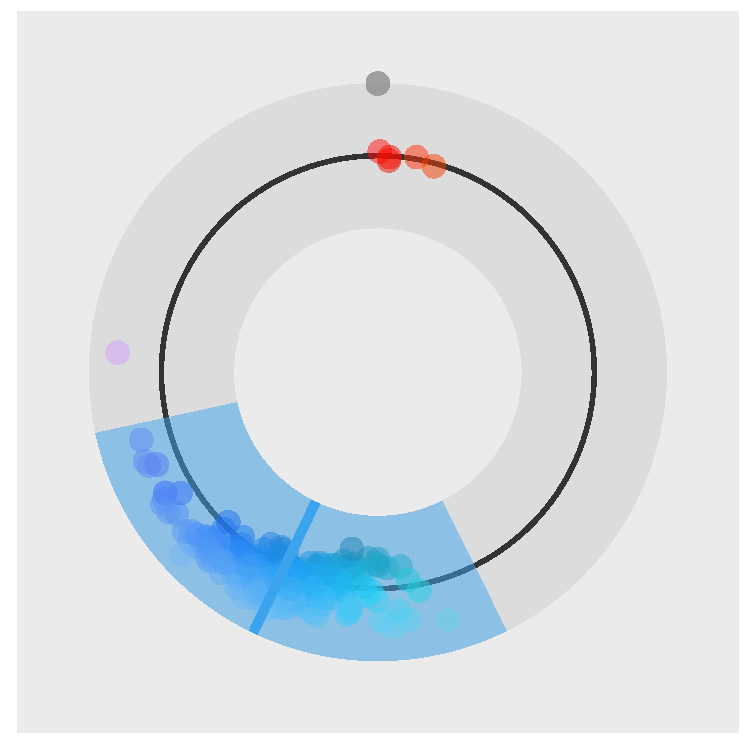
\includegraphics[width=\linewidth]{single_column.pdf}
	\caption{\textbf{A random visualization.} This is an example of a figure that spans only across one of the two columns.}
	\label{fig:column}
\end{figure}

On the other hand, \figurename~\ref{fig:whole} is an example of a figure that spans across the whole page (across both columns) of the report.

% \begin{figure*} makes the figure take up the entire width of the page
\begin{figure*}[ht]\centering
	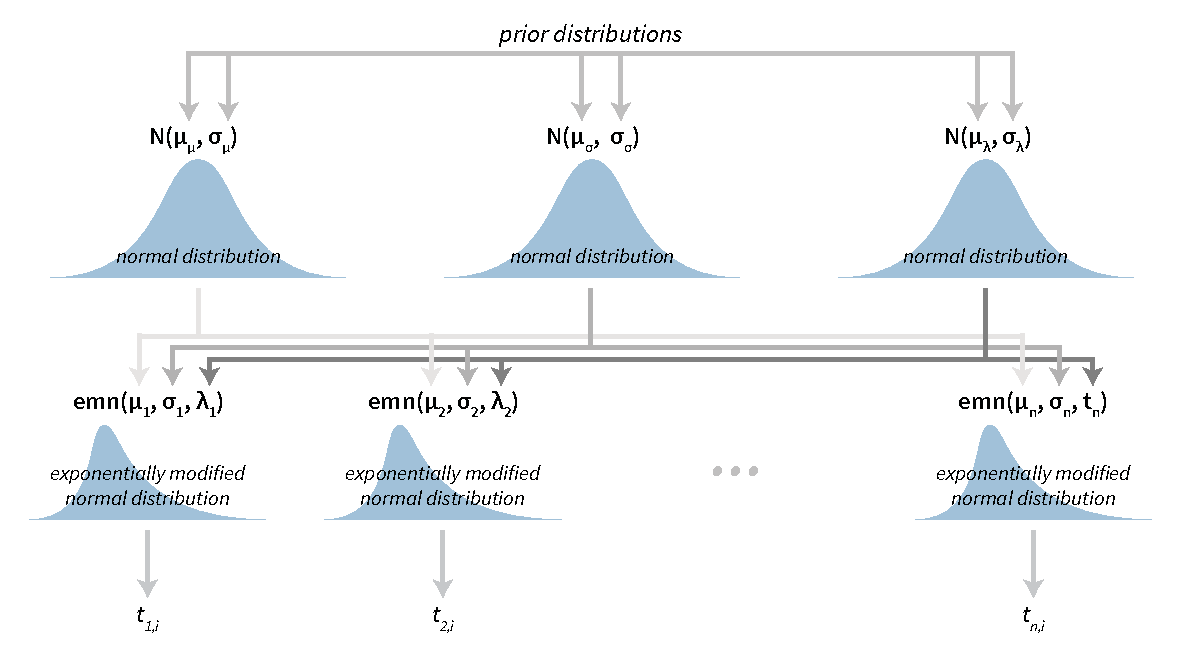
\includegraphics[width=\linewidth]{whole_page.pdf}
	\caption{\textbf{Visualization of a Bayesian hierarchical model.} This is an example of a figure that spans the whole width of the report.}
	\label{fig:whole}
\end{figure*}


\subsection*{Tables}

Use the table environment to insert tables.

\begin{table}[hbt]
	\caption{Table of grades.}
	\centering
	\begin{tabular}{l l | r}
		\toprule
		\multicolumn{2}{c}{Name}       \\
		\cmidrule(r){1-2}
		First name & Last Name & Grade \\
		\midrule
		John       & Doe       & $7.5$ \\
		Jane       & Doe       & $10$  \\
		Mike       & Smith     & $8$   \\
		\bottomrule
	\end{tabular}
	\label{tab:label}
\end{table}


\subsection*{Code examples}

You can also insert short code examples. You can specify them manually, or insert a whole file with code. Please avoid inserting long code snippets, advisors will have access to your repositories and can take a look at your code there. If necessary, you can use this technique to insert code (or pseudo code) of short algorithms that are crucial for the understanding of the manuscript.

\lstset{language=Python}
\lstset{caption={Insert code directly from a file.}}
\lstset{label={lst:code_file}}
\lstinputlisting[language=Python]{code/example.py}

\lstset{language=R}
\lstset{caption={Write the code you want to insert.}}
\lstset{label={lst:code_direct}}
\begin{lstlisting}
import(dplyr)
import(ggplot)

ggplot(diamonds,
	   aes(x=carat, y=price, color=cut)) +
  geom_point() +
  geom_smooth()
\end{lstlisting}

%------------------------------------------------

\section*{Results}

\todo{After the 1st phase}

Use the results section to present the final results of your work. Present the results in a objective and scientific fashion. Use visualisations to convey your results in a clear and efficient manner. When comparing results between various techniques use appropriate statistical methodology.

\subsection*{More random text}

This text is inserted only to make this template look more like a proper report. Lorem ipsum dolor sit amet, consectetur adipiscing elit. Etiam blandit dictum facilisis. Lorem ipsum dolor sit amet, consectetur adipiscing elit. Interdum et malesuada fames ac ante ipsum primis in faucibus. Etiam convallis tellus velit, quis ornare ipsum aliquam id. Maecenas tempus mauris sit amet libero elementum eleifend. Nulla nunc orci, consectetur non consequat ac, consequat non nisl. Aenean vitae dui nec ex fringilla malesuada. Proin elit libero, faucibus eget neque quis, condimentum laoreet urna. Etiam at nunc quis felis pulvinar dignissim. Phasellus turpis turpis, vestibulum eget imperdiet in, molestie eget neque. Curabitur quis ante sed nunc varius dictum non quis nisl. Donec nec lobortis velit. Ut cursus, libero efficitur dictum imperdiet, odio mi fermentum dui, id vulputate metus velit sit amet risus. Nulla vel volutpat elit. Mauris ex erat, pulvinar ac accumsan sit amet, ultrices sit amet turpis.

Phasellus in ligula nunc. Vivamus sem lorem, malesuada sed pretium quis, varius convallis lectus. Quisque in risus nec lectus lobortis gravida non a sem. Quisque et vestibulum sem, vel mollis dolor. Nullam ante ex, scelerisque ac efficitur vel, rhoncus quis lectus. Pellentesque scelerisque efficitur purus in faucibus. Maecenas vestibulum vulputate nisl sed vestibulum. Nullam varius turpis in hendrerit posuere.

Nulla rhoncus tortor eget ipsum commodo lacinia sit amet eu urna. Cras maximus leo mauris, ac congue eros sollicitudin ac. Integer vel erat varius, scelerisque orci eu, tristique purus. Proin id leo quis ante pharetra suscipit et non magna. Morbi in volutpat erat. Vivamus sit amet libero eu lacus pulvinar pharetra sed at felis. Vivamus non nibh a orci viverra rhoncus sit amet ullamcorper sem. Ut nec tempor dui. Aliquam convallis vitae nisi ac volutpat. Nam accumsan, erat eget faucibus commodo, ligula dui cursus nisi, at laoreet odio augue id eros. Curabitur quis tellus eget nunc ornare auctor.


%------------------------------------------------

\section*{Discussion}


\todo{After the 1st phase}

Use the Discussion section to objectively evaluate your work, do not just put praise on everything you did, be critical and exposes flaws and weaknesses of your solution. You can also explain what you would do differently if you would be able to start again and what upgrades could be done on the project in the future.


%------------------------------------------------

\section*{Acknowledgments}

\todo{After the 1st phase}

Here you can thank other persons (advisors, colleagues ...) that contributed to the successful completion of your project.


%----------------------------------------------------------------------------------------
%	REFERENCE LIST
%----------------------------------------------------------------------------------------
\bibliographystyle{unsrt}
\bibliography{report}


\end{document}